\section{Web Application}
%% (Reihenfolge noch vorläufig)
%% - Was ist Django?
%% - Wie setzt Django das MVC-Pattern um?
%% - Installation einschließlich Dependencies
%% - Benutzung der App (allgemein und Admin-Interface)
%% - Tests
%% - Deployment
%% - Datenmodell (Ähnlichkeiten / Unterschiede zum XML-Schema)
%% - Zukünftige Erweiterungen (Templates und Views für Endnutzer,
%%   XML-Export, MySQL/Postgres backend)

\emph{Author: Tim Krones} \\

In addition to functionality for extracting and annotating the
contents of the Sbr-Regesten, the package also provides the basic
architecture for a web application. This chapter gives an overview of
the Django Framework for developing web applications. It then describes
how to

\begin{itemize}
\item install necessary dependencies
\item run the application
\item use the admin interface to add or change data
\end{itemize}

and provides basic pointers for extending and deploying the
application. Also included is a detailed description of the data model
used for storing information extracted from the Sbr-Regesten in the
database associated with the application.

Please note that the purpose of this chapter is to provide a mostly
high-level \emph{overview} of all the different aspects involved in
dealing with Django applications in general, and with the Sbr-Regesten
Web Application in particular. While the information it contains about
how to use the application is quite detailed, some of the other
aspects (for which the Django documentation provides in-depth
coverage) are touched on only briefly. We do give pointers to external
documentation wherever necessary. Therefore, if you have never worked
with Django, this chapter will give you a basic understanding of the
architecture of a Django project, but it is not to be understood as a
replacement for reading the official Django documentation.

\subsection{The Django Web Framework}
\label{sec:django}

The information in this section is based on the official Django
documentation which can be found at
\url{https://docs.djangoproject.com/}.

Django is a Python Framework for rapid prototyping and development of
interactive web applications. It uses the MVC pattern to separate the
different tasks that are involved in creating interactive web
applications.

\subsubsection{The MVC Pattern}
\label{sec:mvc}

\href{https://en.wikipedia.org/wiki/Model_view_controller}{Model-View-Controller},
or MVC for short, is a
\href{https://en.wikipedia.org/wiki/Software_design_pattern}{Software Design Pattern}

commonly used by Web Frameworks such as Django and Ruby on Rails. The
basic idea of MVC is is to divide application logic into three layers.
The \emph{Model} layer is responsible for storing and operating on
data. This usually involves at least the basic
\href{https://en.wikipedia.org/wiki/CRUD}{CRUD} operations
\emph{Create}, \emph{Read}, \emph{Update}, and \emph{Delete}.The
\emph{View} layer takes care of presenting available data to end
users. \emph{Controllers} are responsible for handling user requests.
Depending on the type of request, this usually involves querying the
model layer for data, manipulating this data in various ways (if
necessary), and sending it off to the view layer for presentation.

Different frameworks interpret MVC in different ways; the next chapter
describes Django's implementation of this pattern.

\subsubsection{How Django Implements MVC}
\label{sec:django-mvc}

This chapter presents an overview of how Django interprets and
implements the MVC pattern. For an in-depth treatment of the
individual components, please consult the documentation at
\url{https://docs.djangoproject.com/}.

While Django's seperation of concerns is heavily influenced by the MVC
pattern conceptually, the framework uses a different terminology to
distinguish the individual components for dealing with (user)
requests, data, and presentation. The terminological differences tend
to confuse users that are new to Django or to working with MVC
frameworks in general, which makes it all the more important to
understand these differences before delving into Django development.

Django distinguishes between \emph{models}, \emph{templates}, and
\emph{views}, which is why the framework is commonly referred to as an
``MTV'' framework. The model layer in Django corresponds to the
concept of a model layer as it is defined (or at least commonly
understood) in the context of MVC. Django templates correspond to
views in MVC, and the responsibilities of Django views are similar to
those of controllers in MVC.

From an architectural point of view, a Django \emph{project} usually
consists of one or more Django \emph{apps}. Among other things, each
app includes a dedicated Python module for the model layer (called
\texttt{models.py}), two Python modules that are jointly responsible for
handling user requests (called \texttt{views.py} and \texttt{urls.py})
and a hierarchy of templates written in Django's template language.

The \texttt{models.py} module contains specialized Python classes
(called \emph{models}) which define the data model of a given Django
app. Each class corresponds to a table in the database of the project,
with additional tables being created as necessary to represent
relationships between different models.

The \texttt{views.py} module contains specialized Python functions
(called \emph{view functions}) for handling user requests. These
functions are responsible for querying the database for information,
manipulating that information if necessary, and rendering the
appropriate templates back to the user, filled with the information
that was requested. In this context, the \texttt{urls.py} module acts
as a kind of \emph{dispatcher}: It contains a mapping from URLs (or,
generally speaking, URL patterns) to appropriate view functions,
allowing Django to identify the actions it needs to take based on the
URL that was requested by the user.

\subsection{Installing and Using the Web Application}
\label{sec:webapp}

This chapter explains how to install and use the Sbr-Regesten Web
Application, and also provides some pointers on how to extend and
deploy it.

\subsubsection{Installation}
\label{sec:install}

\paragraph{Python and Django}
The Sbr-Regesten Web Application was developed using Python 2.7.3 and
Django 1.4.3.

Python binaries and source code for all major operating systems can be
obtained from \url{http://python.org/download/}. Python binaries are
usually pre-installed on Linux distributions, and different versions
can be obtained from standard repositories using a package manager:
Please note that at the time of this writing, Django is \textbf{not}
compatible with Python 3, so in order to run the app successfully,
Python 2.7.* needs to be installed.

The easiest way to install specific versions of Django is using the
\href{http://www.pip-installer.org/en/latest/}{pip-installer} which is
a tool for installing and managing Python packages. \texttt{pip}
should be available in the standard repositories of most Linux
distributions (package: python-pip). For generic installation
instructions, visit
\url{http://www.pip-installer.org/en/latest/installing.html}.

Once \texttt{pip} has been installed, version 1.4.3 of Django can be
installed using the following command:

\begin{verbatim}
$ pip install Django==1.4.3
\end{verbatim}

For instructions on how to install Django manually, consult
\href{https://www.djangoproject.com/download/}{this part} of the
Django documentation.

\paragraph{BeautifulSoup}
The process of extracting and annotating information from the
Sbr-Regesten makes heavy use of a tool called \emph{BeautifulSoup},
which needs to be installed in order to reproduce the extraction
process locally.

Like Django, BeautifulSoup is pip-installable:

\begin{verbatim}
$ pip install beautifulsoup4
\end{verbatim}

For the purpose of improving or extending the extraction process,
detailed information about BeautifulSoup can be found in its
\href{http://www.crummy.com/software/BeautifulSoup/bs4/doc/}{official documentation}.

\paragraph{Further Recommendations}
In addition to the hard dependencies described in the previous
sections, we recommend installing the \emph{IPython} interpreter as it
provides a lot of features not included in the standard python
interpreter and thus makes interacting with the database from Django's
development shell a lot easier. The latest version of IPython can be
installed using pip as follows:

\begin{verbatim}
$ pip install ipython
\end{verbatim}

\subsubsection{Running the Application}
\label{sec:run}

Once all necessary dependencies are installed, you are ready to run a
local instance of the application. Extract the contents of the source
archive to an appropriate folder in your file system and \texttt{cd}
into the root folder of the project. This folder is called
\texttt{sbr-regesten}. Look for a file called
\texttt{sbr-regesten.db}. If it's there, this means that the source
package you have received includes a prepopulated database, and that
you can run the application right away by typing

\begin{verbatim}
$ python manage.py runserver
\end{verbatim}

If you find that the database file is missing from the source archive,
you need to proceed as follows: First, initialize the database by running

\begin{verbatim}
$ python manage.py syncdb
\end{verbatim}

At some point you will be asked whether or not you would like to
create a superuser for the database. Type \texttt{yes} and press
Enter, then provide a username, email address and password. For
development purposes it is both convenient and acceptable to simply
set username and password to \texttt{admin}.

When the \texttt{syncdb} command finishes, you can either start using
the application with an empty database by typing the
\texttt{runserver} command listed above, or you can go ahead and
populate the database with information from the Sbr-Regesten. Since
the extraction process was implemented as a Django \emph{management command},
you can trigger it using the following command:

\begin{verbatim}
$ python manage.py extract
\end{verbatim}

Note that this process might take a long time to finish.

\subsubsection{Using the Application}
\label{sec:use}

After starting the development server with the \texttt{runserver}
command, direct your browser to \url{http://127.0.0.1:8000/admin} to
access the application. You will be greeted by a login form:

\begin{figure}[h]
  \centering
  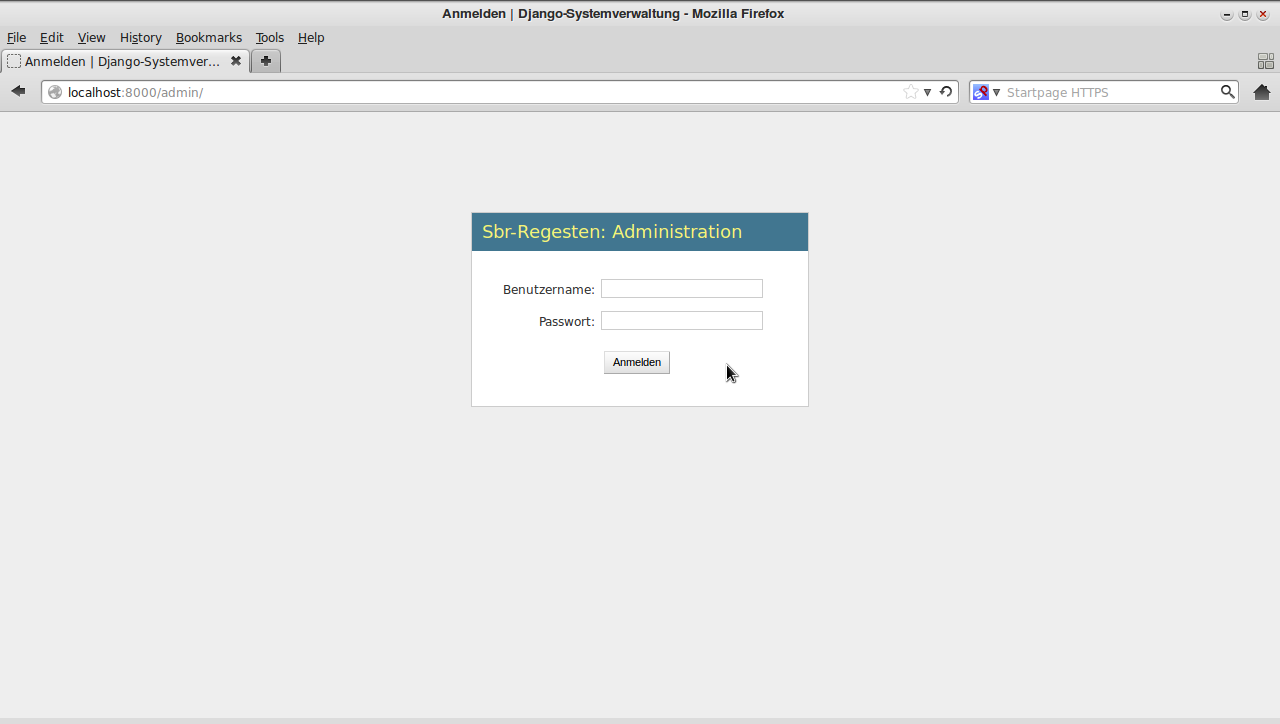
\includegraphics[scale=0.3]{img/admin-login}
  \caption{Login screen for the Django admin interface}
  \label{fig:admin-login}
\end{figure}

If you are working with a prepopulated database, enter \texttt{admin}
in both the \emph{Benutzername} and the \emph{Passwort} field. If you
initialized the database yourself, use the credentials you specified
in the \texttt{syncdb} step explained in the previous section.
Clicking on \emph{Anmelden} will take you to the main page of the
\emph{Django Admin Interface}:

\begin{figure}[h]
  \centering
  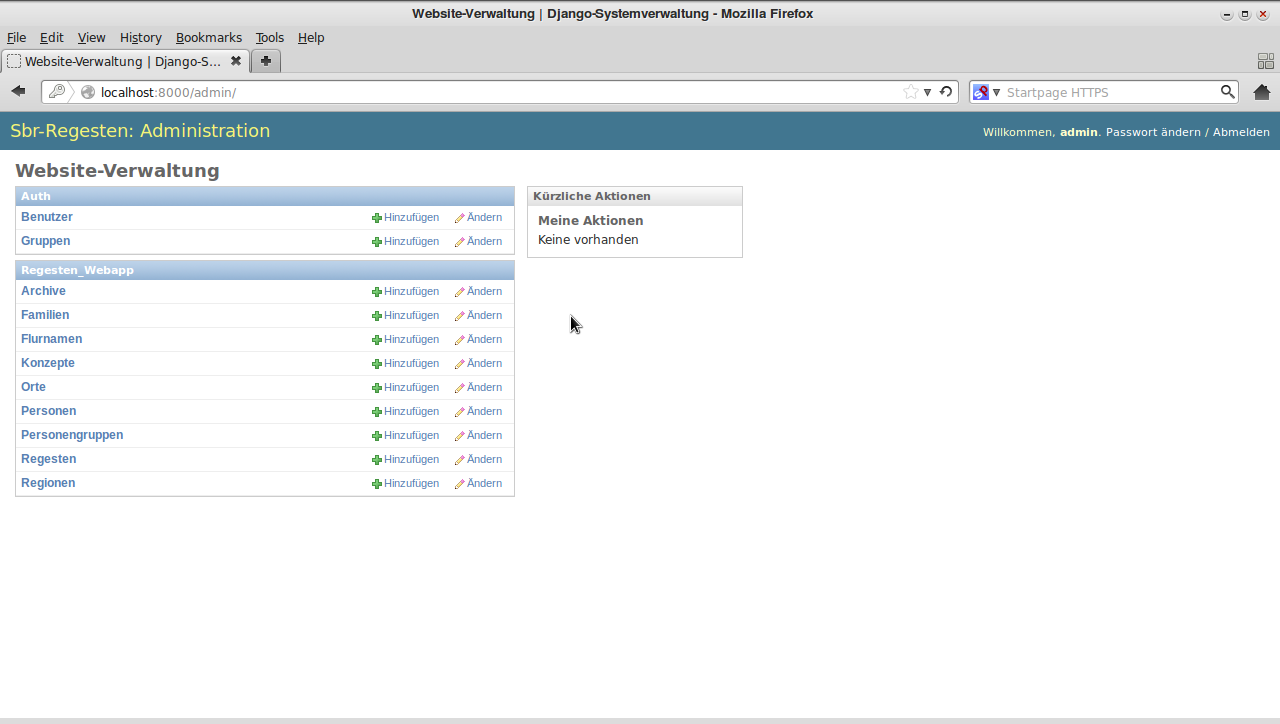
\includegraphics[scale=0.3]{img/admin-main}
  \caption{Main page of the admin interface, starting point for actions described below}
  \label{fig:admin-main}
\end{figure}

The admin interface allows you to browse, search and manipulate (i.e.
add, change, and delete) the data that is stored in the database from
the convenience of your browser.

\paragraph{Browsing and Searching Data}
From the main page of the admin interface you can get listings of
database entries for the following entities that can be found in the
Sbr-Regesten\footnote{Consult chapter \ref{sec:data-model} for more
  information about these entities.}:

\begin{itemize}
\item Archives (listed as \emph{Archive})
\item Families (listed as \emph{Familien})
\item Landmarks (listed as \emph{Flurnamen})
\item Concepts (listed as \emph{Konzepte})
\item Locations (listed as \emph{Orte})
\item Persons (listed as \emph{Personen})
\item Person groups (listed as \emph{Personengruppen})
\item Regests (listed as \emph{Regesten})
\item Regions (listed as \emph{Regionen})
\end{itemize}

Click on the name of a specific entity to get to the corresponding
listing of database entries. The listing for locations (\emph{Orte})
looks like this:

\begin{figure}[h]
  \centering
  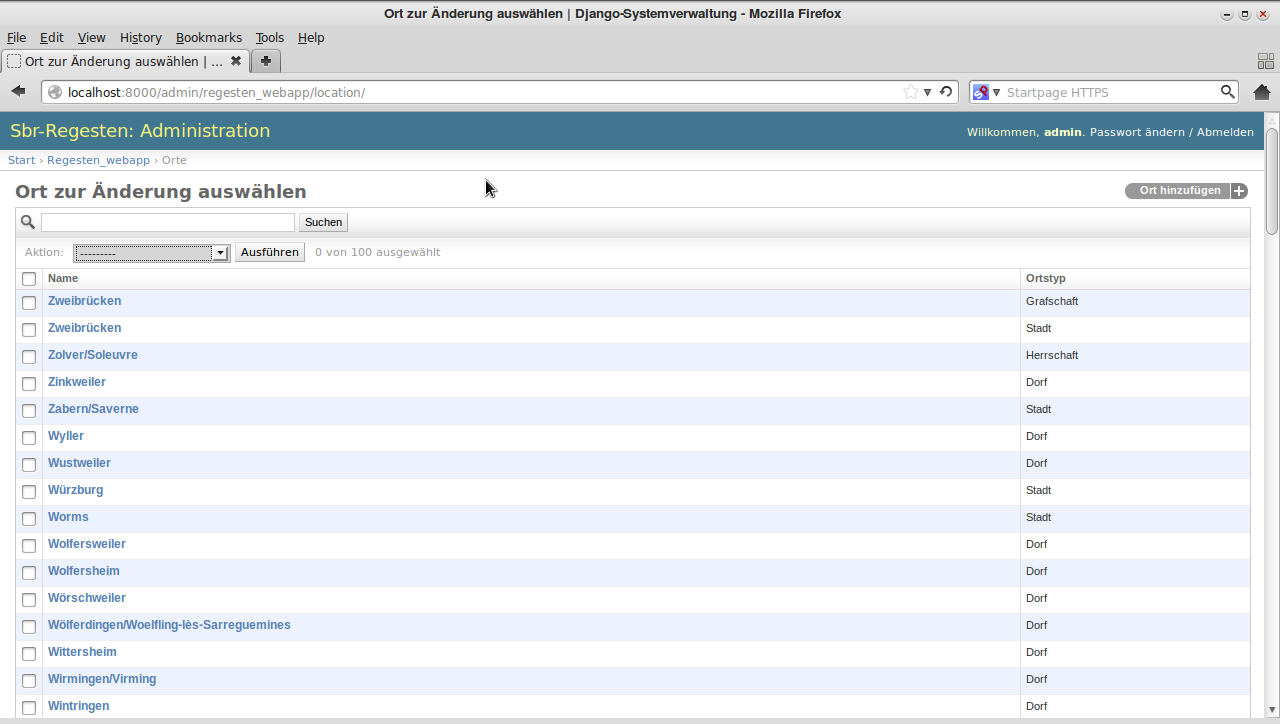
\includegraphics[scale=0.3]{img/admin-loc-listing}
  \caption{Example listing of database entries}
  \label{fig:admin-loc-listing}
\end{figure}

To sort the table by a specific column, click on its header. Clicking
more than once will toggle between ascending and descending order for
that column.

If you are looking for a specific entry, you can narrow down the list
by entering appropriate search terms in the search field and clicking
the \emph{Suchen} button. On the result page, click on the link next
to the information about the number search results to get back to the
full listing.

Note that for efficiency reasons, search is configured to consult only
a limited number of model fields for each entity.

\paragraph{Adding Data}
Starting from the main page of the admin interface, you can manipulate
the data in the database in various ways. For each entity/model that
has been configured to be editable via the admin interface, Django
displays two buttons; one for adding a new database entry for a
specific model (\emph{Hinzufügen}), and another one for changing
information associated with existing entries (\emph{Ändern}).

To add a new database entry for a specific model, click on the
corresponding \emph{Hinzufügen} button. This brings up the appropriate
input form for the model. For instance, the (top part of the) form for
adding a new Regest entry to the database looks like this:

\begin{figure}[h]
  \centering
  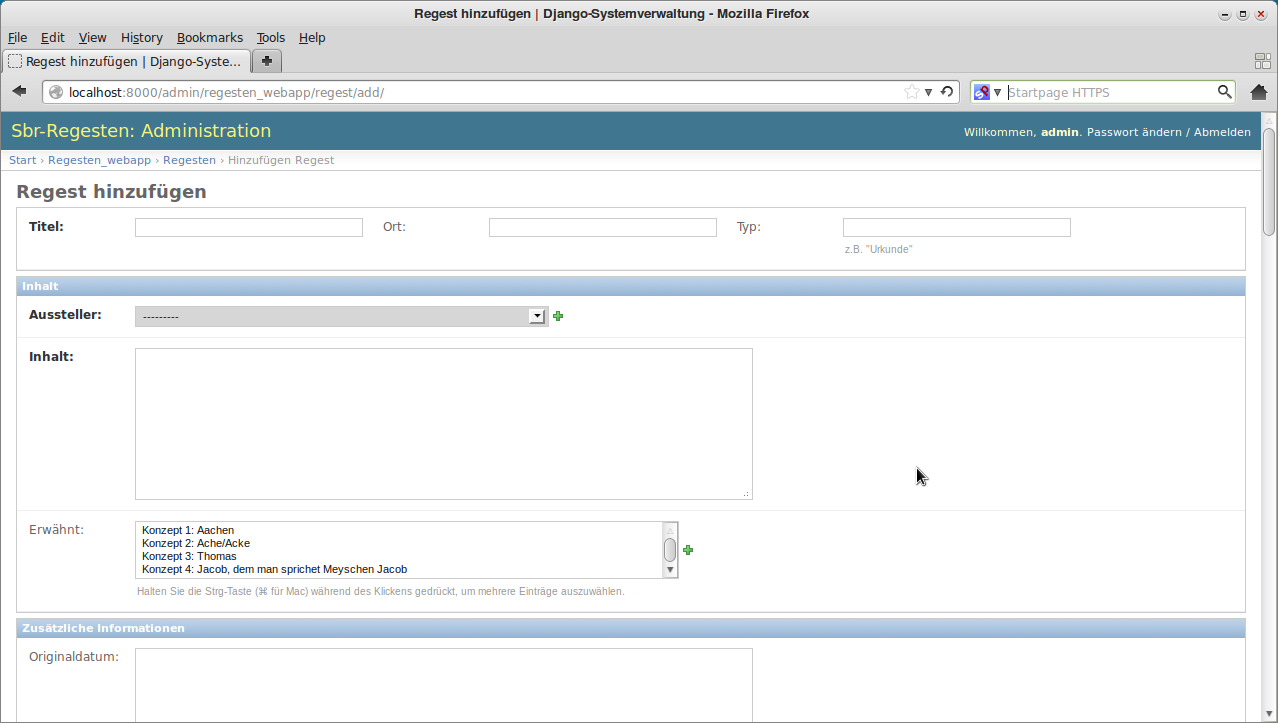
\includegraphics[scale=0.3]{img/add-regest}
  \caption{Example interface for adding a new entry to the database}
  \label{fig:add-regest}
\end{figure}

In any input form, fields with labels in bold font are mandatory. This
means that Django will not allow you to save a new entry to the
database without filling them in. Instead, it will annotate the fields
you failed to fill in with appropriate error messages and redisplay
the input form\footnote{The interface behaves in exactly the same way
  if you \textbf{edit} the information for an existing entry and
  (accidentally) delete any mandatory information.}:

\begin{figure}[h]
  \centering
  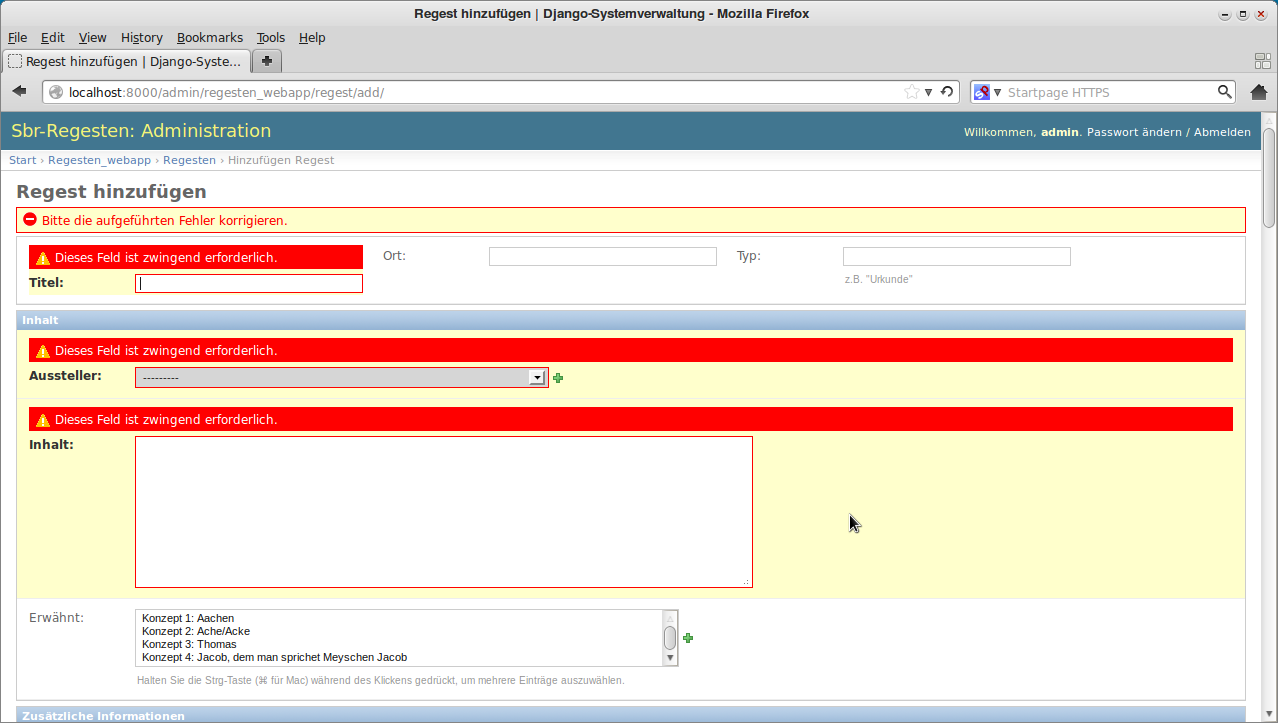
\includegraphics[scale=0.3]{img/add-regest-fail}
  \caption{Input form with errors}
  \label{fig:add-regest-fail}
\end{figure}

When you are done filling in the information that you would like to
store as a new entry in the database, click the \emph{Sichern} button
at the very bottom of the input form. This will take you back to the
listing of existing entries for the model that you were working on.
Alternatively, if you want to add another database entry for the same
model, click the \emph{Sichern und neu hinzufügen} button. This will
bring up a new input form for the same model. If you want to save the
entry and continue working on it afterwards, click \emph{Sichern und
  weiter bearbeiten}.\footnote{Note that this won't work if any of the
  mandatory fields are empty.}

If you are familiar with the Sbr-Regesten, most of the fields included
in the input forms for the different models should be
self-explanatory. Some of the less obvious fields are annotated with
examples of the type of input that they expect. However, before
starting to add or edit information from the admin interface, please
refer to chapter \ref{sec:data-model} to get a more detailed
understanding of the type of information represented by any given
field.

\paragraph{Manipulating Data}
The steps that are involved in editing existing data are very similar
to the ones that are required for adding new entries. On the main page
of the admin interface, click on the \emph{Ändern} button that
corresponds to the type of model you would like to edit one or more
entries for. This will bring up the already familiar listing of
database entries for the model. If necessary, sort or narrow down the
list as described above, then click on the name of the entry you would
like to edit. The fields of the input form that comes up will be
prepopulated with the information that is available for this entry.
Other than that it looks and behaves exactly like the form you are
already used to for adding new entries.

To get a list of all changes that were made to a specific database
entry via the admin interface, click on the button that says
\emph{Geschichte} in the top right corner of the input form.

\paragraph{Removing Data}
If you want to remove a specific entry from the database, navigate to
its input form as described above. Then, on the very bottom of the
page, click the \emph{Löschen} button. This will bring up a
confirmation page that looks like this:

\begin{figure}[h]
  \centering
  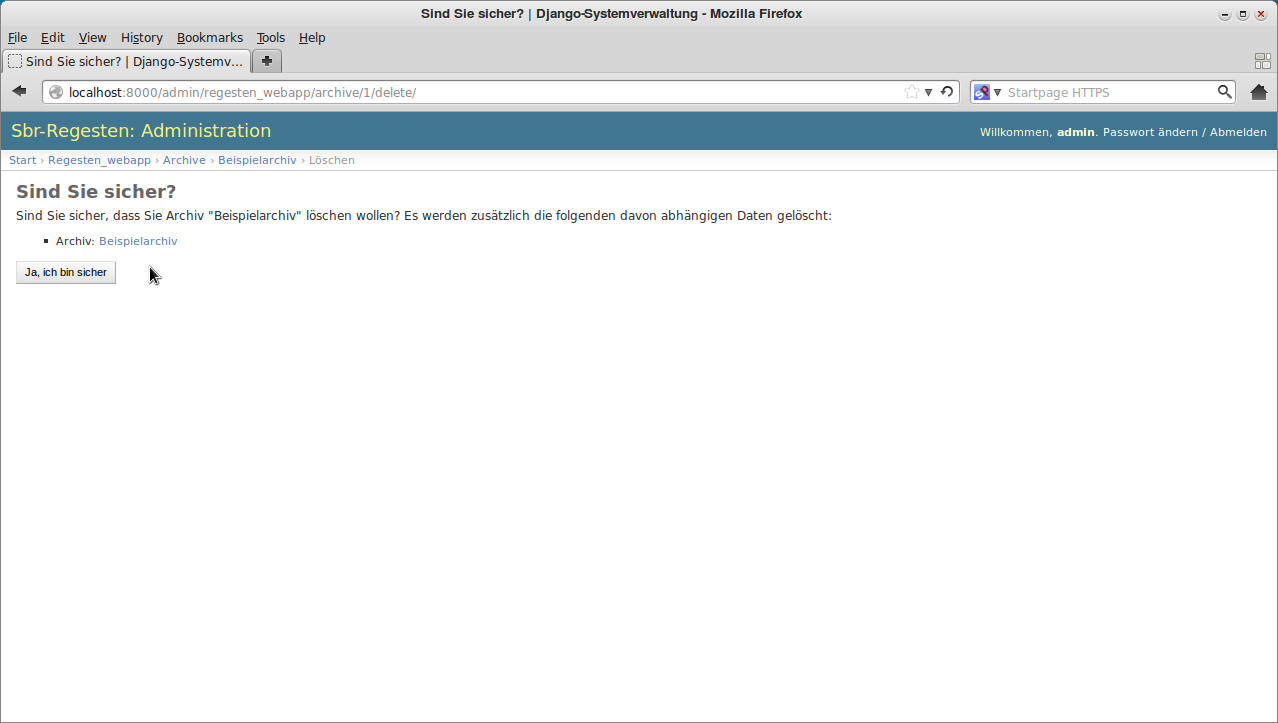
\includegraphics[scale=0.3]{img/confirm-delete}
  \caption{Confirmation page for deleting items}
  \label{fig:confirm-delete}
\end{figure}

Click on the \emph{Ja, ich bin sicher} button to finalize the action.
If you change your mind, you can use e.g. the breadcrumbs to navigate
somewhere else.

It is also possible to delete multiple entries at once. On the page
that lists all existing entries for a given model, mark the entries
you would like to delete by clicking on the checkboxes next to the
names of the entries. Then choose \emph{Ausgewählte MODEL\_NAME
  löschen} from the drop-down menu labeled \emph{Aktion} at the top
and click the \emph{Ausführen} button:

\begin{figure}[h]
  \centering
  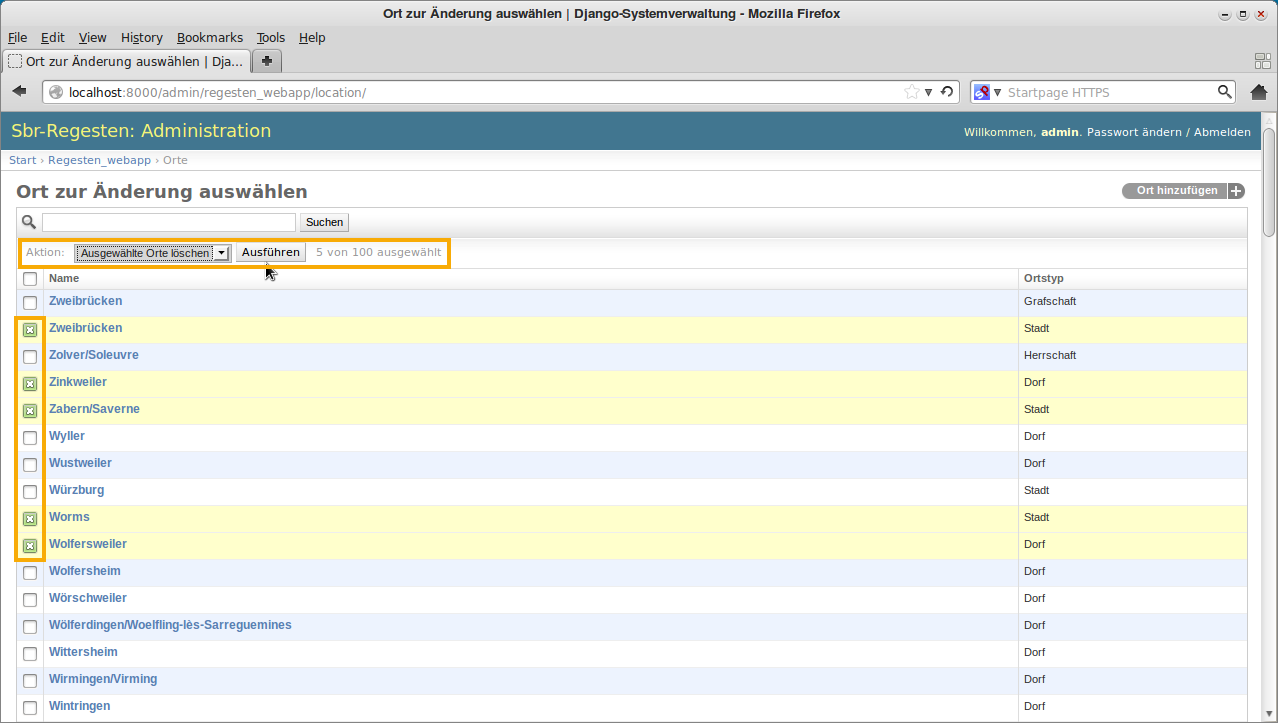
\includegraphics[scale=0.3]{img/delete-multiple}
  \caption{Deleting multiple items at once}
  \label{fig:delete-multiple}
\end{figure}

\subsection{Deployment}
\label{sec:deploy}

As mentioned in section \ref{sec:use}, the \texttt{runserver} command
runs the \emph{development} server for the Sbr-Regesten Web
Application. There are some additional steps you need to take to get
the application set up and running on a production server. Depending
on the type of server you are running, there are several ways to
achieve this, so when you are ready to deploy the application, please
consult the
\href{https://docs.djangoproject.com/en/1.4/howto/deployment/}{Deploying
  Django} section of the Django documentation for detailed information
on different ways to get the application running on your server.

\paragraph{A Note on Debug Mode}

Despite not going into detail here about how to deploy the
Sbr-Regesten Web Application, there is one important security issue
that needs to be addressed: For the purpose of making applications
easy to develop and debug, Django provides a \emph{debug mode}. If
this mode is turned on, Django displays a debug page for any errors or
exceptions that occur while interacting with the application in the
browser. This page includes a full error traceback containing
extensive information about the environment the application is running
in. This poses a high security risk, as it provides users (who might
have malicious intentions) with information they should not have
access to. Therefore, before deploying the Sbr-Regesten Web
Application in a production environment, make sure that the
\texttt{DEBUG} variable (which is used to turn debug mode on and off)
is set to \texttt{False} in
\texttt{sbr-regesten/sbr\_regesten/settings.py}.

\subsection{Extending the Web Application}
\label{sec:extend}

This section provides information about how to obtain a copy of the
source code for development purposes that includes the complete
history of changes. It also includes information about translating the
application, as well as some suggestions about missing features that
should be implemented next.

\subsubsection{Version Control with Git}
\label{sec:git}

The Sbr-Regesten Web Application was developed using the
\href{http://git-scm.com/}{Git Distributed Version Control System}.
For the purpose of extending the application we recommend you continue
using this system, as this will enable you to make use of the
development history in various ways.

\paragraph{Installing Git}

Git is available for all major operating systems. On most major Linux
distributions it can be installed from the standard repositories using
a package manager. For detailed platform-specific instructions and/or
to download graphical installers for MacOS X and Windows, go to
\url{http://git-scm.com/downloads}.

\paragraph{Using Git to Download the Source Code}

The source code repository for the Sbr-Regesten is hosted on
\href{https://github.com/}{GitHub} at
\url{https://github.com/itsjeyd/sbr-regesten}. To obtain a copy of the
most recent version of the source code, \texttt{cd} to the directory
in which you want to store it and enter the following command:

\begin{verbatim}
$ git clone https://github.com/itsjeyd/sbr-regesten.git
\end{verbatim}

This will download (\emph{clone}) the repository to a folder called
\texttt{sbr-regesten} in your current working directory.

Note that doing this will \textbf{not} give you \emph{push access} to
the GitHub repository: Git lets you commit any future changes you make
to the source code \emph{locally}; hosting code on a remote server is
not necessary in order to successfully keep it under version control
with Git. However, unless you are granted permission by the owner of
the GitHub repository, you will not be able to \emph{push} your
changes back to the server.

If you would like to host your own copy of the source code on GitHub
(e.g. to facilitate collaboration among multiple developers), instead
of cloning the code from the original repository, you
should follow these steps:

\begin{enumerate}
\item \href{https://github.com/plans}{Create a GitHub account}
\item \href{https://help.github.com/articles/fork-a-repo}{Fork} the
  original repository
\item Clone the repository from your own fork to your local machine,
  using the \texttt{clone} command above with the appropriate URL.
\end{enumerate}

\paragraph{Git Resources}
There is a wealth of information about how to use Git available
online, so it does not make sense to duplicate this information here.
If you are new to Version Control with Git, the following resources
will help you get started:

\begin{itemize}
\item \href{http://try.github.com/levels/1/challenges/1}{tryGit}, a
  free, \emph{no-setup-required}
  CodeSchool\footnote{\url{http://www.codeschool.com/}} course that
  lets you practise working with Git in the comfort of your browser
\item \href{http://git-scm.com/book}{Pro Git} by Scott Chacon, a
  comprehensive book about Git that is available both in print and
  online; the link references the online version which is searchable
  and continuously receives updates
\item The \href{http://gitref.org/}{Git Reference},
  \begin{quote}
    ``a quick reference for learning and remembering the most
    important and commonly used Git commands'',
  \end{quote}
  which also provides links to relevant sections of the Pro Git book.
\end{itemize}

\subsubsection{Next Steps: Suggestions for Future Extensions}
\label{sec:next}

Before creating a full-fledged web application for the Sbr-Regesten, a
data model to represent the contents of the original document had to
be created. This task was the main focus of our project, along with
extracting, annotating and storing the information contained in the
Sbr-Regesten based on this new model. The purpose of this section is
to point out functionality that was outside the scope of this project
but should most likely be implemented next.

\paragraph{Changing the Database Backend}

Django supports a number of different database engines. By default it
uses \emph{sqlite3}, as this involves virtually no additional setup,
because Python 2.7 includes sqlite connector modules in its standard
library. For development purposes, sqlite is an acceptable choice. In
terms of performance, however, it leaves a lot to be desired and is
therefore not recommended for use in a production environment.
\href{http://www.mysql.com/}{MySQL} and
\href{http://www.postgresql.org/}{PostgreSQL} are much more suited for
these kinds of environments.

There are several steps involved in changing the database backend:

\begin{enumerate}
\item If you haven't already, install the database engine of your
  choice on the server you are planning to deploy on
\item Install the appropriate Python bindings for the type of database
  you picked
\item Grant Django the necessary rights to create and alter tables;
  for testing purposes, Django will also need permission to create
  test databases
\item Change the \texttt{ENGINE} option in the \texttt{DATABASES}
  constant in \texttt{settings.py} to the value corresponding to the
  new engine.
\end{enumerate}

For additional information, refer to the
\href{https://docs.djangoproject.com/en/1.4/topics/install/#database-installation}{Get
your database running} section of the Django documentation.

\paragraph{XML Export}

As new information gets added to the database via the admin interface
of the web application, the XML version of the Sbr-Regesten will
become more and more outdated. In order to prevent this, a feature
that allows for XML export of database entries needs to be
implemented. In the spirit of
\href{https://en.wikipedia.org/wiki/CRUD}{CRUD}, this could e.g. be
done by adding entity-specific \texttt{to\_xml} methods to each of the
relevant models. Additionally, for convenience sake, this
functionality could be integrated into the admin interface by writing
a custom
\href{https://docs.djangoproject.com/en/1.4/ref/contrib/admin/actions/}{Admin
  Action}. Admin actions are useful for performing the same task on
multiple database entries at once; for example, deleting multiple
database entries is an instance of an admin action. They are available
from the drop-down menu labeled \emph{Actions} on the pages that list
existing entries for individual models (see section \ref{sec:use},
``Browsing and Searching Data'').

\paragraph{Public Pages for End-Users}

In terms of actual functionality, the web application so far ``only''
provides an interface for \emph{administrating} the information stored
in the database. Regular users will most likely not be given access to
this interface, and the Django Admin Interface was also not designed
to be used by a large number of end users. The application is lacking
functionalities for (presenting the information stored in the database
to) end users, which will have to be implemented before releasing the
application to the public. In more technical terms, this means that
future work will focus heavily on the \emph{view} and \emph{template}
layers of the application.

The following sections of the Django documentation provide detailed
information about these layers:

\begin{itemize}
\item
  \href{https://docs.djangoproject.com/en/1.4/topics/http/}{Handling
    HTTP requests}
\item
  \href{https://docs.djangoproject.com/en/1.4/topics/forms/}{Working
    with forms}
\item
  \href{https://docs.djangoproject.com/en/1.4/topics/templates/}{The
    Django template language}
\end{itemize}

\subsubsection{Adding Tests for New Features}
\label{sec:test}

Django comes with a built-in test execution framework which extends
the \texttt{unittest} module included the Python Standard Library for
web development-specific needs. By default, when using the
\texttt{startapp} management command to create the basic structure for
a new Django app, Django creates a single module for the tests
associated with the app called \texttt{tests.py}. This module is
located in the top-level directory of the app. However, as individual
apps grow in size, it might become necessary to split up their tests
into several modules to keep the overall architecture modular. Django
provides support for this: If you create a directory called
\texttt{tests} on the same level as the default \texttt{tests.py}
module, you can put as many test modules in this directory as you
like, and you can name them whatever you want, without the need for
any additional setup.

The current version of the Sbr-Regesten Web Application already
includes tests for non-trivial methods of the model layer. They are
located in the default \texttt{tests.py} module under
\texttt{sbr-regesten/regesten\_webapp/}. To run them, issue the
following command from the top-level directory of the \emph{project}:

\begin{verbatim}
$ python manage.py test regesten_webapp
\end{verbatim}

The Django framework itself also comes with a large number of tests.
To run tests for all built-in Django apps that the Sbr-Regesten
project uses, along with the tests that are currently defined in
\texttt{sbr-regesten/regesten\_webapp/tests.py}, you can use the
following command:

\begin{verbatim}
$ python manage.py test
\end{verbatim}

When extending the Sbr-Regesten Web Application, tests for any new
features of the model layer (e.g. XML export) can be added to the
existing \texttt{tests.py} module. As soon as you start implementing
views and templates for end users, however, we recommend that you
switch to using a dedicated \texttt{tests} directory and multiple test
modules as described above.

To learn more about about writing and running tests for Django
applications as well as using alternative testing frameworks, consult
the
\href{https://docs.djangoproject.com/en/1.4/topics/testing/}{Testing
  Django applications} section of the official Django documentation.

\subsubsection{Internationalization: Translating the Application}
\label{sec:translate}

As the Sbr-Regesten Web Application is targeted at users whose native
language is German, any new functionality associated with user-facing
features will require translation. Django provides comprehensive
support for internationalization and localization that can be
leveraged to make this process easy.

The basic procedure for translating relevant parts of a Django
application consists of the following steps:

\begin{enumerate}
\item Add translation hooks to the code where necessary; these hooks
  are also called \emph{translation strings}
\item Extract translation strings into a \emph{message file}
\item Add translations for the individual strings to the message file
\item Compile the message file
\end{enumerate}

In regular Python code, translation strings are specified using the
\texttt{ugettext()} function, which by convention is imported as
\texttt{\_}. As an example, consider the definition of the
\texttt{title} attribute of the \texttt{Regest} model:

\begin{verbatim}
title = models.CharField(_('title'), max_length=70)
\end{verbatim}

The first argument to the \texttt{models.CharField} constructor is the
\emph{verbose name} of the attribute to use for presentation purposes.
By default, Django uses the name of the attribute (with underscores
converted to spaces) as its verbose name, but for the purpose of
telling Django that we want it to translate the name of this
attribute, we have to specify it in the constructor, and surround it
with a call to \texttt{ugettext()} / \texttt{\_}. Looking at the
remaining definition of the Regest model and other model definitions
in \texttt{models.py}, you will notice many more examples for
translation strings.

To update the message file for German translations of the code base
when you are done implementing a new feature, run the following
command from the \texttt{sbr-regesten/regesten\_webapp} directory:

\begin{verbatim}
$ django-admin.py makemessages -l de
\end{verbatim}

The message file for German translations is located in the directory

\begin{verbatim}
sbr-regesten/regesten_webapp/locale/de/LC_MESSAGES
\end{verbatim}

and it is called \texttt{django.po}. To add translations for new
translation strings open this file and fill all empty \texttt{msgstr}
strings with the appropriate translations. The structure of message
files is explained in detail in the Django documentation (see below
for a link).

As a last step, when you (or your translators) are done editing the
message file, you need to compile it by running the following command
from the same directory you ran the \texttt{makemessages} command from
earlier:

\begin{verbatim}
$ django-admin.py compilemessages
\end{verbatim}

This command outputs a compiled message file called \texttt{django.mo}
to the \texttt{LC\_MESSAGES} directory that also holds the plain text
version of the message.

Finally, please note that Django uses the GNU \texttt{gettext}
utilities for creating and compiling message files. If these utilities
are not available, the files generated by the \texttt{makemessages}
command will be empty.

To learn more about Django's features for translating applications,
consult the
\href{https://docs.djangoproject.com/en/1.4/topics/i18n/}{Internationalization
  and localization} section of the official documentation.

\subsection{Django Data Model}
\label{sec:data-model}

\subsubsection{Regesten}
\label{sec:reg-model}

\subsubsection{Index}
\label{sec:index-model}
